\documentclass{standalone}
\standaloneconfig{border=2mm 2mm 2mm 2mm}
\usepackage{tikz}
\usepackage{amsmath}
\usetikzlibrary{calc}

\begin{document}

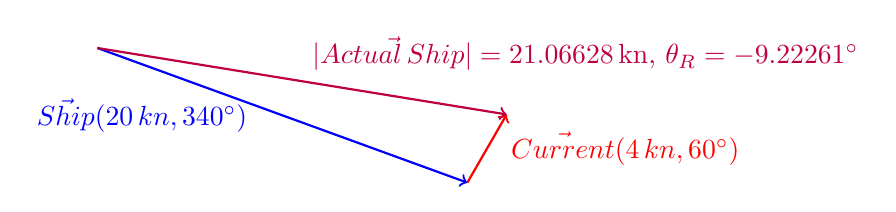
\begin{tikzpicture}[scale=0.25]
    % Define the origin
    \coordinate (O) at (0,0);
    
    % Define the polar coordinates (magnitude and angle) of each vector
    \def\mA{20}    % Magnitude of vector A
    \def\angleA{340} % Angle of vector A (degrees)

    \def\mB{4}    % Magnitude of vector B
    \def\angleB{60} % Angle of vector B (degrees)

    \def\mC{0}    % Magnitude of vector C
    \def\angleC{0} % Angle of vector C (degrees)
    
    % Convert polar coordinates to Cartesian for each vector endpoint
    \pgfmathsetmacro{\Ax}{\mA*cos(\angleA)}
    \pgfmathsetmacro{\Ay}{\mA*sin(\angleA)}

    \pgfmathsetmacro{\Bx}{\mB*cos(\angleB)}
    \pgfmathsetmacro{\By}{\mB*sin(\angleB)}

    \pgfmathsetmacro{\Cx}{\mC*cos(\angleC)}
    \pgfmathsetmacro{\Cy}{\mC*sin(\angleC)}
    
    % Calculate the resultant vector components
    \pgfmathsetmacro{\xR}{\Ax + \Bx + \Cx}
    \pgfmathsetmacro{\yR}{\Ay + \By + \Cy}
    
    % Calculate the magnitude and angle of the resultant vector
    \pgfmathsetmacro{\mR}{sqrt((\xR)^2 + (\yR)^2)}
    \pgfmathsetmacro{\angleR}{atan2(\yR, \xR)}

    % Define coordinates for A, B, C, and R
    \coordinate (A) at (\Ax, \Ay);
    \coordinate (B) at (\Bx, \By);
    \coordinate (C) at (\Cx, \Cy);
    \coordinate (R) at (\xR, \yR);
    
    % Draw vectors A, B, C from the origin
    \draw[->, thick, blue] (O) -- (A) node[midway, left=9pt] {$\vec{Ship} (\mA\,kn, \angleA^\circ)$};
    \draw[->, thick, red] (A) -- ++(B) node[midway, right=5pt] {$\vec{Current} (\mB\,kn, \angleB^\circ)$};
    %\draw[->, thick, green] (A) ++ (B) -- ++(C) node[midway, above=5pt] {$\vec{C} (\mC, \angleC^\circ)$};
    
    % Draw the resultant vector R from the origin
    \draw[->, thick, purple] (O) -- (R) node[midway, above right] {$|\vec{Actual\,Ship}| = \mR$\,kn, $\theta_R = \angleR^\circ$};
\end{tikzpicture}

\end{document}
